\section{ISAC 中的性能权衡}

本节将探讨 ISAC 中的性能权衡，包括信息论极限、物理层性能、传播信道和跨层指标等方面的权衡。我们首先介绍基本的 S\&C 性能指标，然后深入分析它们之间的联系和权衡关系。

\subsection{感知与通信 (S\&C) 性能指标}

感知任务大致可分为三类：检测 (Detection)、估计 (Estimation) 和识别 (Recognition)。这些任务均基于从感知对象获取的信号或数据来完成 \cite{10.1145/3310194}。尽管这些术语在不同应用场景和协议层中可能具有不同的含义和实现方式，本文将其定义如下。


\paragraph{1) 检测 (Detection)}
检测是指在存在噪声和/或干扰的观测条件下，对感知对象的状态做出二元或多元决策。此类状态通常包括：目标的有/无（物理层），以及某一事件是否发生（应用层），例如运动检测，这可以建模为二元或多假设检验问题。以二元检测为例，我们基于观测信号在两个假设 $\mathcal{H}_1$ 和 $\mathcal{H}_0$ 之间进行选择（例如：目标存在或不存在）。检测指标包括\textit{检测概率}（定义为当 $\mathcal{H}_1$ 成立时检测器选择 $\mathcal{H}_1$ 的概率）和\textit{虚警概率}（表示当 $\mathcal{H}_0$ 成立时检测器却选择了 $\mathcal{H}_1$ 的概率）\cite{kay1998fundamentals}。

\paragraph{2) 估计 (Estimation)}

估计是指在存在噪声和（或）干扰的观测条件下，从接收信号中提取感知目标的有用参数。这些参数包括目标的距离、速度、角度、数量以及尺寸等信息。

估计性能通常通过均方误差 (Mean Squared Error, MSE) 和克拉美罗下界 (Cramér-Rao Bound, CRB) 进行评估 \cite{restuccia2021ieee}。均方误差定义为参数真实值 $\theta$ 与其估计值 $\hat{\theta}$ 之间误差平方的期望：
\begin{equation}
	\mathrm{MSE} = \mathbb{E} \left[ (\theta - \hat{\theta})^2 \right].
\end{equation}
MSE 越小，表明估计精度越高。

克拉美罗下界 (CRB) 表示任意无偏估计器方差能够达到的理论下限，其定义为费舍尔信息 (Fisher Information, FI) 的倒数：
\begin{equation}
	\mathrm{CRB} = \frac{1}{I(\theta)},
\end{equation}
其中 $I(\theta)$ 表示参数 $\theta$ 的费舍尔信息。费舍尔信息定义为似然函数关于参数 $\theta$ 的曲率（负二阶导数）的期望值，用于衡量观测数据所包含的信息量以及估计器的精度。

\paragraph{3) 识别 (Recognition)}

识别是指根据含有噪声和（或）干扰的观测数据判断感知对象的类别或属性。这类任务包括目标识别、人类活动识别以及事件识别等。识别通常被建模为应用层的分类 (Classification) 问题，其性能主要通过识别准确率 (Recognition Accuracy) 进行评估 \cite{tait2005introduction}。识别准确率定义为：
\begin{equation}
	\mathrm{Accuracy} = \frac{N_{\text{correct}}}{N_{\text{total}}},
\end{equation}
其中 $N_{\text{correct}}$ 表示正确分类的样本数量，$N_{\text{total}}$ 表示总样本数量。

\paragraph{总结}
对于物理层感知任务而言，检测概率、虚警概率、均方误差以及克拉美罗下界是最重要的性能评价指标。而对于高层应用中的感知任务，特别是基于机器学习的方法，识别准确率则是衡量系统性能的核心指标。此外，更复杂的感知任务（例如无线成像）通常需要对复杂目标执行多次检测和估计操作，因此其性能评价往往需要综合考虑检测与估计两类指标。

\subsection{信息论极限}

信息论为评估 ISAC 系统的基本性能界限提供了严谨的理论支撑。其核心目标是揭示通信速率与感知精度之间的帕累托（Pareto）最优边界。

\begin{figure}[htbp]
	\centering
	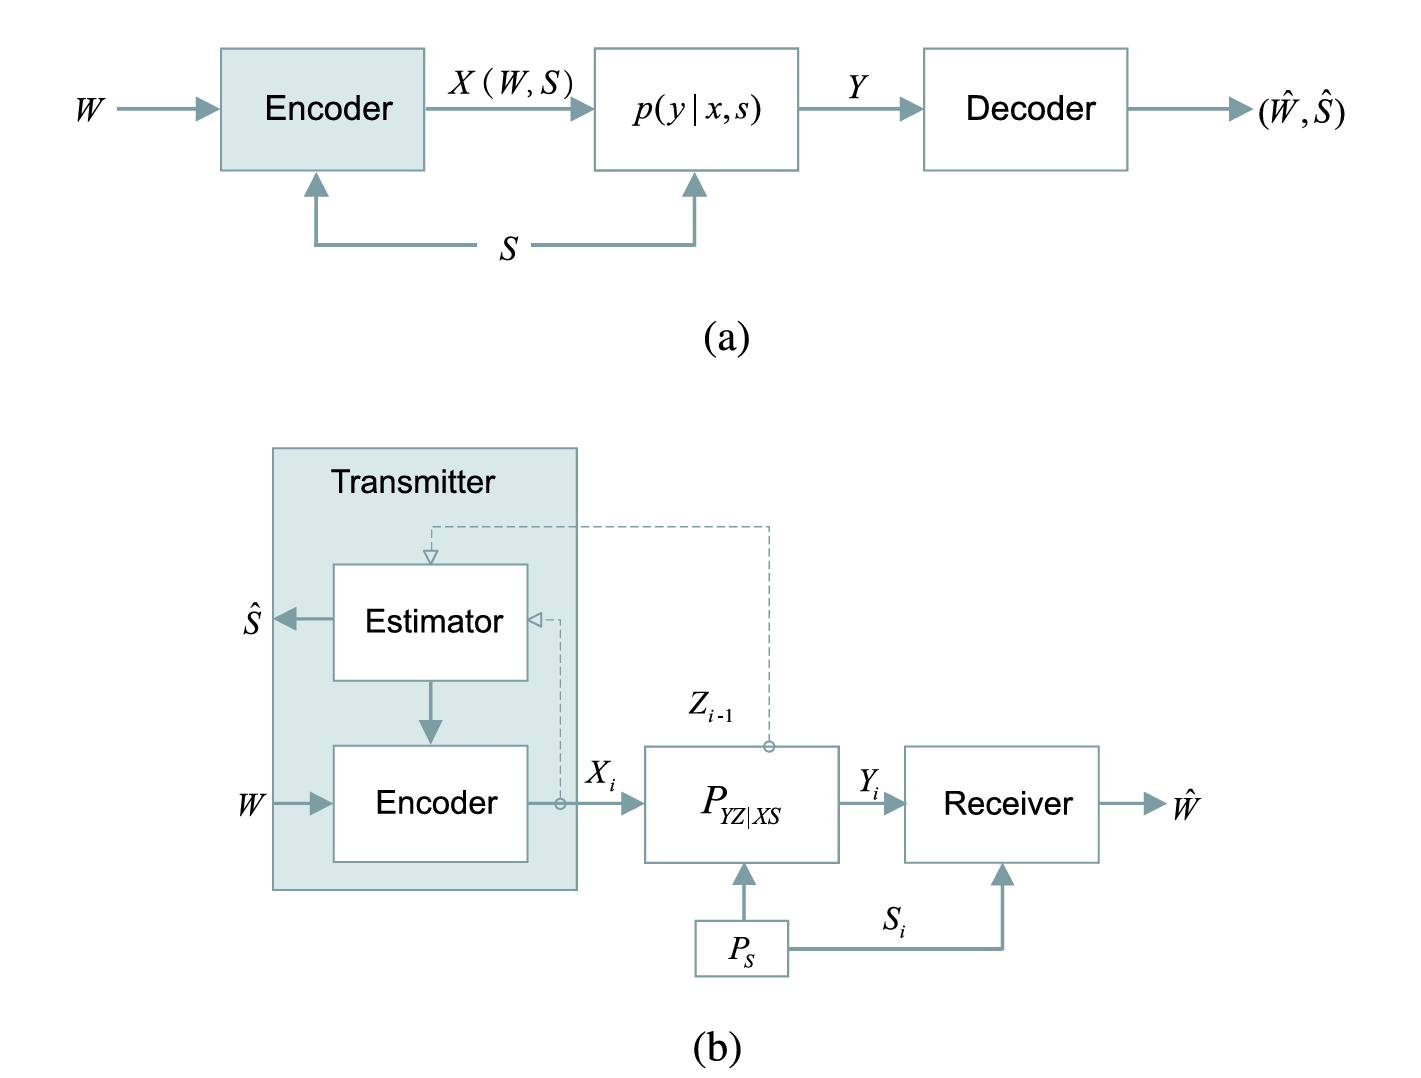
\includegraphics[width=0.6\linewidth]{img/3-1.png}
	\caption{（a）通过状态相关信道进行信息传输；（b）单基地ISAC信道：通过具有广义反馈的状态相关信道进行信息传输。}
	\label{fig:3-1}
\end{figure}


这张图片展示了从信息论角度定义的集成感知与通信（ISAC）数学模型。它将感知任务建模为对“信道状态”（State）的估计。以下是针对两幅子图的详细解释：

图 (a) 展示了状态相关信道上的通用 ISAC 模型，其特点是感知任务主要在接收端完成。在该模型中，发送端编码器将待传信息 $W$ 与预知的环境状态 $S$（如目标位置信息）映射为发射信号 $X(W,S)$，信号经由受状态 $S$ 影响的信道 $p(y|x,s)$ 传输至接收端。接收端的解码器需承担双重任务：一方面恢复原始通信数据 $\hat{W}$，另一方面根据收到的信号 $Y$ 反推环境状态 $\hat{S}$。该模型的核心意义在于从信息论层面揭示了在共享同一信号资源的前提下，通信传输速率与感知估计精度之间存在的理论折衷关系。

图 (b) 描述了更具工程参考价值的单站 (Mono-static) ISAC 信道模型，其感知任务由发射端通过反馈机制实现。发送端集成了编码器与估计器，前者将信息 $W$ 编码为信号 $X_i$ 发射，后者则通过接收来自信道的广义反馈 $Z_{i-1}$（即雷达回波信号）来实时估计环境状态 $\hat{S}$。信道 $P_{YZ|XS}$ 在环境状态 $P_S$ 的作用下产生两路输出：一是传向远端接收机用于解码 $\hat{W}$ 的通信信号 $Y_i$，二是反射回发送端用于感知探测的回波信号 $Z_i$。该模型强调了基站通过“自发自收”机制实现原生的感知功能，而远端终端则仅需专注于通信数据的接收与处理。

\qquad

其中，最著名的理论成果是 I-MMSE 关系式 \cite{1412024}，它建立了通信互信息 $I$ 与感知最小均方误差 (MMSE) 之间的优雅联系：
\begin{equation}
	\frac{d}{d\mathrm{snr}} I(\mathrm{snr}) = \frac{1}{2} \mathrm{MMSE}(\mathrm{snr}). \label{eq:1}
\end{equation}
该式揭示了通信速率对信噪比的导数恰好等于 MMSE 的一半。从物理意义上讲，这说明能最大化通信速率的高斯分布输入反而会导致感知的 MMSE 达到最大，从而量化了 S\&C 性能在底层信号统计特性上的根本矛盾。

进一步地，ISAC 性能极限可通过容量--失真（Capacity-Distortion）权衡框架来评估 \cite{936166}。在状态相关的高斯信道 $Y = X(W, S) + S + N$ 下，通过功率共享（Power-sharing）策略，可推导出 $(R, D)$ 对的闭式帕累托边界：
\begin{equation}
	(R, D) = \left( \frac{1}{2} \log \left( 1 + \frac{\gamma P}{Q_N} \right), \frac{Q_S ( \gamma P + Q_N )}{ ( \sqrt{Q_S} + \sqrt{(1-\gamma)P} )^2 + \gamma P + Q_N } \right), \label{eq:6}
\end{equation}
其中 $\gamma \in [0, 1]$ 为功率分配因子，用于控制通信信息传递与感知状态估计之间的资源权衡。

针对更复杂的单站雷达感知场景，由于发射机无法预知目标状态，研究者将其建模为延迟反馈信道。在此框架下，容量--失真折衷 $C(D)$ 可描述为如下优化问题：
\begin{equation}
	C(D) = \max_{P_X} I(X; Y \mid S), \quad \text{s.t. } \mathbb{E} \{ d(S, \hat{S}) \} \leq D. \label{eq:8}
\end{equation}
该公式定义了在满足感知失真约束 $D$ 的前提下所能达到的最大通信速率。对于此类非闭式优化问题，通常采用改进的 Blahut-Arimoto (BA) 算法 \cite{8437621}进行数值求解，以获得特定信道环境下的帕累托前沿。

Blahut-Arimoto (BA) 算法是信息论中一个非常经典的数值计算算法。它由 Richard Blahut 和 Suguru Arimoto 在 1972 年独立提出，主要用于解决以下两类基本问题：

1. 计算信道容量 ($C$)：在已知信道统计特性（转移概率）的情况下，寻找最优的输入分布以达到最大传输速率。

2. 计算率失真函数 ($R(D)$)：在给定允许的失真限度下，寻找最有效的源编码方案。

